%%%%%%%%%%%%%%%%%%%%%%%%%%%%%%%%%%%%%%%%%%%%%%%%%%%%%%%%%%%%%%%%%%%%
%% I, the copyright holder of this work, release this work into the
%% public domain. This applies worldwide. In some countries this may
%% not be legally possible; if so: I grant anyone the right to use
%% this work for any purpose, without any conditions, unless such
%% conditions are required by law.
%%%%%%%%%%%%%%%%%%%%%%%%%%%%%%%%%%%%%%%%%%%%%%%%%%%%%%%%%%%%%%%%%%%%

\documentclass[
  digital, %% This option enables the default options for the
           %% digital version of a document. Replace with `printed`
           %% to enable the default options for the printed version
           %% of a document.
  table,   %% Causes the coloring of tables. Replace with `notable`
           %% to restore plain tables.
  nolof,     %% Prints the List of Figures. Replace with `nolof` to
           %% hide the List of Figures.
  nolot,     %% Prints the List of Tables. Replace with `nolot` to
           %% hide the List of Tables.
  nocover
  %% More options are listed in the user guide at
  %% <http://mirrors.ctan.org/macros/latex/contrib/fithesis/guide/mu/fi.pdf>.
]{fithesis3}
%% The following section sets up the locales used in the thesis.
\usepackage[resetfonts]{cmap} %% We need to load the T2A font encoding
\usepackage[T1,T2A]{fontenc}  %% to use the Cyrillic fonts with Russian texts.
\usepackage[
  main=english, %% By using `czech` or `slovak` as the main locale
                %% instead of `english`, you can typeset the thesis
                %% in either Czech or Slovak, respectively.
  english, german, russian, czech, slovak %% The additional keys allow
]{babel}        %% foreign texts to be typeset as follows:
%%
%%   \begin{otherlanguage}{german}  ... \end{otherlanguage}
%%   \begin{otherlanguage}{russian} ... \end{otherlanguage}
%%   \begin{otherlanguage}{czech}   ... \end{otherlanguage}
%%   \begin{otherlanguage}{slovak}  ... \end{otherlanguage}
%%
%% For non-Latin scripts, it may be necessary to load additional
%% fonts:
\usepackage{paratype}
\def\textrussian#1{{\usefont{T2A}{PTSerif-TLF}{m}{rm}#1}}
%%
%% The following section sets up the metadata of the thesis.
\thesissetup{
    date          = \the\year/\the\month/\the\day,
    university    = mu,
    faculty       = fi,
    type          = bc,
    author        = Dominik Gmiterko,
    gender        = m,
    advisor       = Radek Pelánek,
    title         = {Similarity of programming problems},
    TeXtitle      = {Similarity of programming problems},
    keywords      = {similarity, metrics, programming, keyword2, ...},
    TeXkeywords   = {similarity, metrics, programming, keyword2, \ldots},
    abstract      = {This is the abstract of my thesis, which can

                     span multiple paragraphs.},
    thanks        = {These are the acknowledgements for my thesis, which can

                     span multiple paragraphs.},
    bib           = thesis.bib,
}
\usepackage{makeidx}      %% The `makeidx` package contains
\makeindex                %% helper commands for index typesetting.
%% These additional packages are used within the document:
\usepackage{paralist} %% Compact list environments
\usepackage{amsmath}  %% Mathematics
\usepackage{amsthm}
\usepackage{amsfonts}
\usepackage{url}      %% Hyperlinks
\usepackage{markdown} %% Lightweight markup
\usepackage{listings} %% Source code highlighting
\lstset{
  basicstyle      = \ttfamily,%
  identifierstyle = \color{black},%
  keywordstyle    = \color{blue},%
  keywordstyle    = {[2]\color{cyan}},%
  keywordstyle    = {[3]\color{olive}},%
  stringstyle     = \color{teal},%
  commentstyle    = \itshape\color{magenta}}
\usepackage{floatrow} %% Putting captions above tables
\floatsetup[table]{capposition=top}
\begin{document}

%
% Oficialne ZADANI v.1
%
% Cílem práce je prozkoumat metody pro měření podobnosti výukových položek na
% základě dat o odpovědích studentů. Práce navazuje na předchozí výzkum v rámci
% skupiny Adaptive Learning. Cílem práce je kriticky prozkoumat dříve navržené
% metody, zejména s ohledem na nevyjasněné aspekty jejich chování na reálných
% datech (neočekávané pravidelnosti v distribucích hodnot podobnosti). Na
% základě získaného vhledu budou navrženy upravené metody nebo doporučení pro
% praktický postup.
%
%                                                                   KISS
%


\chapter*{Introduction}
\addcontentsline{toc}{chapter}{Introduction}

\begin{markdown*}{%
  hybrid,
  definitionLists,
  footnotes,
  inlineFootnotes,
  hashEnumerators,
  fencedCode,
  citations,
  citationNbsps,
}

% --------------------------- %
% Introduction                %
% --------------------------- %

% interactive educational systems

Tutoring systems are computer-based systems designed to introduce users into various domains.
They usually have large amount of items which enables them to provide personalized experience. To maintain this large pool of items efficiently we need to be able to decide which items are useful and which are not.

% focus on systems with large amount of items

% one possible method, using similarity of items

% goal of this work

% structure of this work

Besides Introduction and Conclusion chapters, this thesis is structured into three additional chapters. First chapter talks in general about problem of measuring similarity of programming problems. It explains difference between program and programming problem, which data we have available and techniques used for measuring similarity of problems. Second chapter advances level deeper and describe everything what is specific to data we used. First part of chapter describes programming environment of Robotanik and data from it. Second part focuses in detail on metrics we used in experiments. Last chapter gives overview of implementation and usage of metrics and their evaluation.

# Similarity

% --------------------------- %
% Similarity                  %
% --------------------------- %

% Intro to chapter

%% Structure

In this chapter we will talk in general about questions in learning systems, and computing their similarity. Most of the chapter focuses on explaining what kinds of data are available when comparing questions in learning systems and techniques to do so. Last section describes goals of the thesis.

%% Using similarity in related fields

A lot of research has been dedicated to similarity in many different fields computer science like bioinformatics (sequence alignment, similarity matrix of proteins), information retrieval (document similarity), plagiarism detection and many more.

%TODO este sme nepovedali ze pouzivame performance, presunut

One closely related area is recommender systems which differs from problem similarity only slightly. Both areas are distinguishing users and items. Only difference is that we know how well user did while solving specific item and recommender systems use rating of the items.

%%% Main difference from educational systems

Main difference is that we can use more data about problem. We also have some problem statement and data about performance of students when solving problem.

## Items

% Items

%% Why this term

In this work we use the term “items” (problems, questions, assignments) when we refer to single entry in educational system which users can answer to. Since many aspects of this work are generally applicable we decided to use this general term. In some learning systems this can refer to simple choice from two options in another complex tasks which user solves in matter of minutes.
On other side of the spectrum are systems for teaching introductional programming. Users tend to spend few minutes solving each task and there is fewer of them.

%% Data sources

To further specify the context of our research, we will describe characteristics of items. For computing similarity of items it is most important knowing which data are available to us. Therefore we describe items by sources of data can be used for measuring similarity.

- **Item statement:** specification of the item that a learner should solve, e.g., as a natural language description of the task.

- **Item solutions:** details about solutions obtained from learners or sample solution to item.

- **Learner's performance:** for example item solving times, correctness of answer, number of attempts needed.

This description of item is broad enough to cover most of learning systems. In next chapters we will discuss two systems in particular - umimecesky a umimematiku.

## Why is similarity of items useful
% Why is similarity of items useful

As we mentioned previously key part of learning solving of educational items.

## Computing similarity of items
% Computing similarity of items

The general approach to measuring and using similarity of educational items

## Used datasets
% Datasets

% types of data (real, simualted), why?, real, simulated

In our analysis we use both real data from educational system and simulated data. There is a reason why use both as only real-world data are useful for concluding any results. However evaluation of this data is often complicated as we do not know truth about many of their aspects. That's why we used simulated data for validating some of our conclusions. We will talk more in depth about how we generated simulated data in next chapter when describing their specific usage.

Most of used real-world data comes from system [Umíme česky](https://umimecesky.cz/). Later we have validated our results by also using data from its sibling system [Umíme matiku](https://umimematiku.cz/). We think it is useful as data come from another context but are provided in same format and therefore can be used directly in previously created tools.

### Umíme česky
% czech grammar, "fill-in-the-blank" with two choices, correctness and time, multiple grammar concepts, example of one exercise

[Umíme česky](https://umimecesky.cz/) is system for practice of Czech grammar. System contains multiple exercise types, but in our analysis we use only one exercise - simple "fill-in-the-blank" with two possible answers. This type of exercise can be then viewed by student in multiple ways.
%TODO all views of exercise

!["fill-in-the-blank" example question](img/umimecesky_doplnovacka)

We focused only on "fill-in-the-blank" exercises but they can still be used to train many concepts of Czech grammar.
%TODO different concepts in grammar

### Umíme matiku


# Evaulation

% --------------------------- %
% Evaulation                  %
% --------------------------- %

% Description of common projection output

%% why is projection useful

it is hard to say anything about data when tehre is a lot of it
we especialy focused on systems which consist of TODO1000s of solvable items and even more users
in cases like this it is not possible to look at data about each item individually
possible with projection of many-dimensional data into 2 dimensions.

%% similarity and projection

In general we want our projection to put similar items together. This can be achieved in many different ways. It is important to choose correct source of data and method of processing them prior to applying dimensionality reduction.

%% how does projection look like, possible answers and levels

\begin{figure}
  \begin{center}
    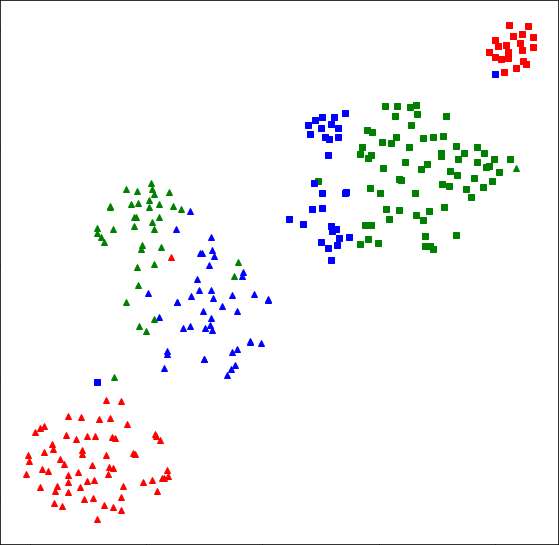
\includegraphics[width=10cm]{img/common_projection}
  \end{center}
  \caption{Basic projection of one knowledge component in Umíme česky}
  \label{fig:commonprojection}
\end{figure}

Figure \ref{fig:commonprojection} shows how common projection looks like. This particular projection shows 273 items of single concept from system. Each item is represented as one dot in the image and its proximity to others represents how similar they are.

## Visible Properties of projection
% Visible Properties of projection

%% Similar words near each other

\begin{figure}
  \begin{center}
    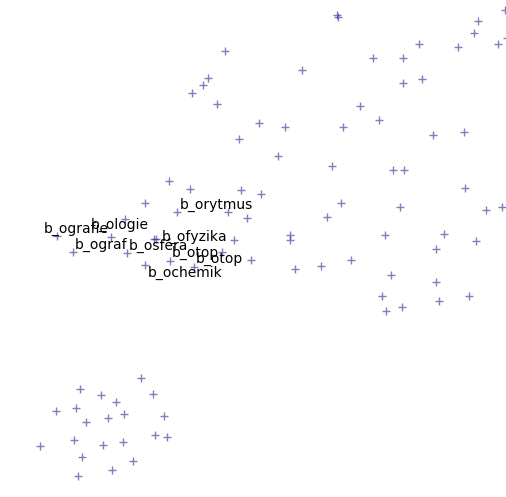
\includegraphics[width=10cm]{img/similar_words}
  \end{center}
  \caption{Similar words close to each other}
  \label{similarwords}
\end{figure}

we want to use results of calculated similarity and projections for managing item pool. That puts some constrains on how ideal results look like.

We want similar items to end as close to each other as possible. When using performance as data source this is especially items using same skill are projected near each other. E.g. figure \ref{similarwords} shows projection of questions about Czech language with highlighted a few similar words. This group consists of words witch are based on single word with added suffix.

%% Regularities

%% This causes similar words to end-up far away one from another

After looking at image you can notice some regularities.

### Computation of item similarity
%% How is projection (similarity) computed

To better understand how was this image created we have to understand how it is computed. We will describe it following section. This is default work-flow we used in most cases. Whenever we don't specify otherwise all projections were produced using this work-flow.

%%% Performance matrix

1. First step we have to do is converting raw logged information about user answers to performance matrix. This matrix consist of entries for each user-item pair. Columns of the matrix are items in educational system and each row of the matrix contains data about single user's performance. In most cases we used correctness of first users answer to specific item as his performance. This means value 1.0 in case of correct answer and 0.0 for incorrect. Another possible choice is to incorporate user solving time into this value. TODO possible choices are described in article [] Performance matrix is relatively sparse as it is not common for users to solve all the items in the system.

I tried using both first users answer and last in performance matrix. However there is no visible difference in resulting projection (same clusters are formed). This is clear when we compare first and last answers of users. There is only 5% difference between them. So at least with large number of items in system it doesn't really matter which one is chosen.

%%% Similarity matrix

2. Next step is computing similarity matrix. Matrix $S$ is square matrix where each position $S_{ij}$ denotes similarity of items $i$ and $j$. In our case similarity is computed as correlation of two columns $i$ and $j$ in performance matrix. This means we look only at users who solved both items $i$ and $j$ and compute Pearson correlation coefficient of their performance.

%%% PCA, (TSNE)

3. The last (optional) step is producing 2D projection. This can be achieved by using many techniques for computing low dimensional projections.

%%%% PCA over TSNE

We choose to use Principal component analysis (PCA) and there is several reasons for doing so.
Result of PCA is deterministic. It produces same result for same input. This is not true for TSNA which is technique using machine learning and gradient descent for finding some local extreme. Stable results are more suitable for understanding data as there is one less variation to results caused by algorithm. It is easier to compare results when altering metrics used fro computing item similarities.

First two principal components of PCA are then used for 2D visualizations.

%%% Why this work-flow, performance data (not item statement)

We choose this specific work-flow as we think it is utilizing data about items which hold most information about their similarity. As other possible choices are item statement and solutions provided by students they do not hold as much information. Item statements in our particular exercises consist only of few Czech words. Also student solution is only choice from two provided options. Item statement and solutions can be used more effectively in other contexts like programming, mathematics, physics, or chemistry.

This choice of work-flow is also relatively simple and easy to understand. It consist of few steps which can be studied separately and interchanged.


## Level regularity
% Level regularity
%% Description of problem, 3 clusters based on 3 levels of questions difficulty

When you look back at figure \ref{fig:commonprojection} you can see that there are three colors of items. Most TODOknowledge components in system Umíme česky are spitted into multiple levels of difficulty. For this particular knowledge component there are three difficulty levels. First level is shown with red, second with green and third blue. This shows visible pattern in our data - each color (level) forms a distinct cluster.  In following section we will try to explain factors that can affect resulting projections produced from real-world data.

As we mentioned before, only data about user performance (correctness of answers) are used when composing projections. And there is not a direct reason for this clusters of same levels to form as no information about belonging to particular level is presented to the algorithm.

%%% cause? how users tend to solve them

Levels are not solved uniformly. It is not common for user to sole all three levels. Less experienced users tend to solve only first or first two levels. However typically older users solve only higher levels. Main cause for this is that system allows teachers to assign particular level of concepts as homework. Students then usually solve only this single level.

%%% why is this unsuitable

%%%% Example of similar words far away one from another

This phenomenon is not suitable for analysis of item similarity as it can cause misleading results. One particular example is when similar word are displayed far away form one another just because they belong to different levels. This is visible for words "bič" and "bičík" in problem set "Vyjmenovaná slova B".

### Sparseness of performance matrix
%% question? can missing data affect result of similarity calculation

%%% Simulated data experiment

For purpose of determining this, we designed an experiment.
writing script that simulated answers provided by virtual students. Main problem we wanted to recreate was missing data in performance matrix. Each simulated user solved level and then with some probability continued to another. So most users answered only to one level, some users to 2 levels and only few to all 3 levels. Levels were chosen at random as users are not required to continue chronologically. Good enough as users do not solve levels in order from easy to hard. There are also users who solve only second or only highest difficulty level.

Results indicate that that structure of data can affect results only in really special cases. But this is not our case. The only case where projection is divided into clusters is when there is absolutely no performance data between any question of groups.

%%% filtered on users who solved 50 of each level

Another approach how to validate this is filtering data leaving only users who solved all levels.
Only if user solved at least 50 questions of each level

So division of questions into 3 levels does not affects similarity of items directly. There is some other factor causing this.

## Different performance metrics
% Different performance metrics

%%% what different measures measure

%% Quantification of level clustering, split and compare with truth

## Answer regularity
% Answer regularity
%% Description of problem, items are divided into clusters based correct answer (i/y) when there is no information about this in data used for computing similarity

%%% TODO Outsider detection using similarity data

When exploring data, it may be useful to detect outsiders. It may be useful for multiple reasons [TODO cite]. In our aprticular case we declare item an outsider when it is not somilar to any other items in problem set.
seems like a logical path to take.

In particular this means item with low sum of similarities to other items may be an outsider. This is where we encountered another regularity in data.

%% Total similarity

 Sum of similarities is sum of one column of simialrity matrix which we produced in our workflow for computing projection.

![Histogram of similarities](i_y_histogram.png)

%%% total similarity histograms by answer

%%% quantification for different concepts

This is not specific to only one problem set (which was used in previous images), almost all problem sets display similar pattern. However for some its more distinct than for others. (Sets consisting of items with many possible answers do not behave this way. But that is to be expected.)


%% Users are choosing one answer by default when they do not know answer

%%% it is usually answer on left, but there are exceptions koncovky pridavnych mien je to Y (v pravo)

%%% how to detect this in performance data? / what can we detect in data?

%% Division of user answers 50-50, but not for correct answers

%% Levels of similarity

## Second level of similarity

Applying one additional level of correlation to item similarity matrix was suggested [TODO].
This means we are looking whether items are behaving similarly with respect to other items instead of similarity of user performance directly.

We can study possible usage of this technique little further

One approach is take a step back, do not use any similarity at all and compute projection directly from performance matrix.
This is usually not useful as performance matrix has large amount of missing values and PCA works only with full matrices.
However it is useful for exploring how adding computation of similarity affects projections.

We used only users who solved all questions.

## Another context
% Another context

%% Replicated in another context of math

%% (re)Usage in other concepts

# Conclusion

% --------------------------- %
% Conclusion                  %
% --------------------------- %



\end{markdown*}

  \makeatletter\thesis@blocks@clear\makeatother
  \phantomsection %% Print the index and insert it into the
  \addcontentsline{toc}{chapter}{\indexname} %% table of contents.
  \printindex

\appendix %% Start the appendices.
\chapter{An appendix}
Here you can insert the appendices of your thesis.

\end{document}
